\chapter{Application concept}

This chapter describes the project plan and the concepts for the developed application. These concepts are foundation of the developed application and describe how the internal processes in the application work.


\section{Project planning}

The project followed the incremental development model. For initial planning the features from existing cost estimation software as described in section \ref{sec:stateofart}. The next step was creating a \textit{GUI prototype} to show how the estimation would look like on a smartphone. Afterwards each cycle followed the rules of incremental development. An evaluation of the wanted features for the application was done in meetings with my supervisor Prof. Dr. Georg Rock. Those features request were compiled into the project goals and requirements. For the next step they were analyzed and implemented. Testing for the application were made afterwards by some of my fellow students. The result was then presented in a meeting and further features were planned for the next iteration cycle.
\begin{figure}[h] 
	\centering 
	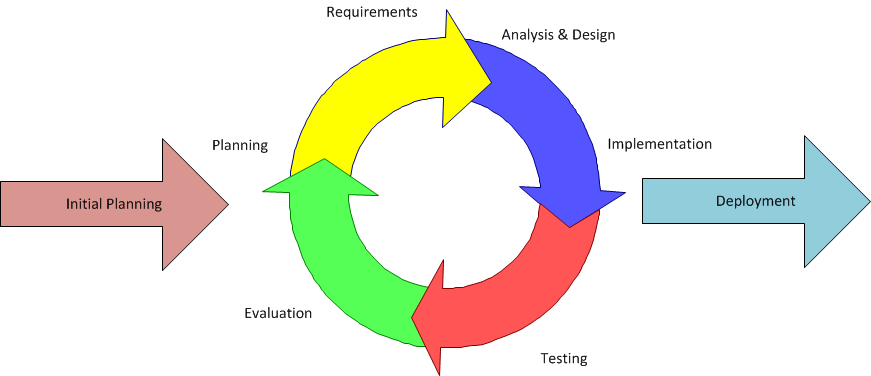
\includegraphics[width=14cm]{images/iterativeDev.PNG} 
	\caption{- Incremental Development} 
	Source: \url{https://www.inflectra.com/Methodologies/}
	\label{fig:incrementaldev}
\end{figure}\\


\subsection{Objectives}\label{objectives}

The project targets are the benefit the application should bring the user. They are linked with the requirements from section \ref{requirements} and describe the condition to be achieved with the application. Whereas requirements can change over time, targets stay the same.\\
Most important target, as described in table \ref{projecttargets}, is \textit{T01}. 'The application must allow a quick and mobile cost estimation of IT Projects' describes that the cost estimation has to be implemented for mobile device use. Also, the cost estimation has to be fast and can use features of the mobile platform to achieve this target.\\
As the developed application is only a beta version, it has to be developed modular for future feature implementation, as described in \textit{T04}.\\
\textit{T06} describes the target that represents an admired feature. The application should provide the possibility to compare projects and measure their relation. This allows to check previous projects for their cost estimation, that the user has a reference how much effort similar projects took.\\
The target for this bachelor thesis is to implement the function point estimation technique. This is the showcase for this application and shows the possibility of cost estimations for software project on mobile devices and is described in \textit{T09}.\\
All remaining targets are medium priority and describe what processes to achieve with this project.\\

\begin{table}[h]
	\centering 
	\setlength{\tabcolsep}{4pt}
	\begin{tabular}{|l||p{14cm}|}\hline
		ID		& Target\\ \hline\hline
		T01  	& The application must allow a quick and mobile cost estimation of IT Projects.\\ \hline
		T02  	& The application must provide informations how cost estimations work.\\ \hline
		T03  	& The application have to improve the cost estimation during  the project life cycle.\\ \hline
		T04  	& The application architecture has to be modular to add new cost estimation methods and analysis tools faster and more efficient.\\ \hline
		T05  	& With the application it is possible to get the information of completed projects and take advantage of their estimation.\\ \hline
		T06  	& The application allows comparison between projects and shows projects that are related to each other.\\ \hline
		T07  	& The application gives information about the estimated man days of a project and the estimated costs.\\ \hline
		T08  	& A project analysis within the application allows an overview of the project changes and gives detailed information about the estimation.\\ \hline
		T09  	& Till the end of the bachelor thesis the function point method has to be implemented and be fully operational.\\ \hline
	\end{tabular} 
	\caption{Project Targets} 
	\label{projecttargets} 
\end{table}

\subsection{Requirements}\label{requirements}

All requirements for the implemented application are based on the targets described in section \ref{objectives} and from the regular meetings. All requirements are described in the appendix XXXX and meet the demands for requirements as described by Balzert \cite{basiskonzepteRE}.\\


\subsection{Cost Estimation}
For the evaluation of the needed time, the project was estimated with the function point technique. Therefor all functionalities are grouped into functional groups, as described by Poensgen \cite{FPKompakt}. Afterwards each function was assigned a category for the estimation, as described in \ref{fpcomponents}.\\
The group Project, as described in \ref{fig:projectFunctionalityGroup}, inherits all functions for a project. All function groups for the application can be found in the application. The project functionalities in \ref{fig:projectFunctionalityGroup} are created with the requirements. Some requirements can be grouped into one functionality. As an example the function \textit{Create/Edit Project} inherits all requirements described in the appendix XXX. This function is marked as an \textit{EI} and \textit{ILF} because all changes are made by the user for this function and creates or edit all internal files for the project. \\
\begin{figure}[h] 
	\centering 
	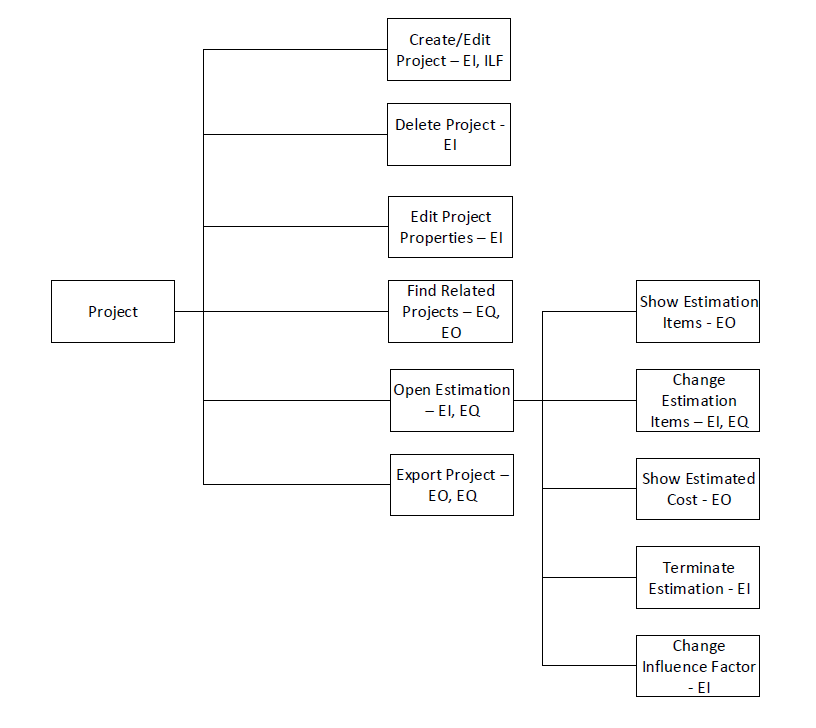
\includegraphics[width=14cm]{images/ScreenOverviewProject.PNG} 
	\caption{- Function Group - Project} 
	\label{fig:projectFunctionalityGroup}
\end{figure}\\
Functions that expects an input from the user are marked as \textit{EI}, like delete project. Output functions like show estimated cost are a \textit{EO} function, because they only display values and results to the user. Functions with a calculation are described as \textit{EQ} combined with \textit{EO} if they produce an output like \textit{Export Project} or process an \textit{Input} like \textit{Change Estimation}.The total functional group can be found in the appendix. This categorization of the function groups was inserted into the estimation table as described in table \ref{estimation:data}.Summed up the project has total \textbf{246} \textit{Function Points}.
\begin{table}[h]
	\centering 
	\setlength{\tabcolsep}{4pt}
	\begin{tabular}{|l|c|c|c|c|}\hline
		Category		&  Amount 		&  Classification	&  Weight 	& Sum of Row\\ \hline
		Input Data   	& 17      		& medium  			& 4			& 68	\\ \hline
		Request Data   	& 6      		& simple  			& 3			& 18	\\ \hline
		Output Data   	& 8      		& medium  			& 5			& 40	\\ \hline
		Dataset   		& 8      		& complex  			& 15		& 120	\\ \hline
		Reference Data  & 0      		& simple  			& 5			& 0	\\ \hline
		\textbf{Sum}   			&       		&   				& 			& \textbf{246}	\\ \hline
	\end{tabular} 
	\caption{Estimation - Total Points} 
	\label{estimation:data} 
\end{table}\\
As described in section \ref{FPMethod}, the next step is to set the influence factors which are described in table \ref{estimation:influence}. The influence factor \textit{Integration into other applications} is set to two because the application has no direct communication to other software. The application does not work with other applications but has local data, like the databases that have to be processed which is the reason for setting the factor \textit{Local Data Processing} to two. As the application is only a local software for the end users device their no much transaction to be excepted. To assure that there is enough time planned to implement a access to the database this factor is set to one. There are many algorithms and equations in the application which have to be checked for errors and exceptions. Also a high effort for the logical component is to be expected. Because of this all influence factors in the \textit{Processing Logic} group are set to the second highest value. For further development of the application a high effort has to be expected for \textit{Reusability} in the project which is the reason for this influence factor to be set at two. There is not much data to be expected from other applications. Only the database cause a higher effort with queries to transform the data from the database in readable informations for the application. Changes in the application can not be made by the user. He can change settings and some appearances which is why this influence factor is set to one. Completed with the equation from \ref{FPMethod} all influence factors result in a multiplier of \textbf{1.01}. Together with the total function points, the influence multiplier is calculated with the equation \ref{fp:TFP} which give \textbf{243.54} points as result. Calculated with the points per day from table \ref{tab:pointsperday} the project is estimated to take \textbf{14} man days. In section \ref{result} it is analyzed how this estimation has worked out and how much time the project took.\\
\begin{table}[h]
	\centering 
	\setlength{\tabcolsep}{4pt}
	\begin{tabular}{|l|c|}\hline
		Influence Factor						&  Weight 	\\ \hline
		Integration into other applications   	& 2      		\\ \hline
		Local Data Processing   				& 2      		\\ \hline
		Transaction Rate   						& 1      		\\ \hline
		Processing Logic   						&       		\\ \hline
		\phantom{ab}- Arithmetic Operation   					& 4      		\\ \hline
		\phantom{ab}- Control Procedure   					& 4      		\\ \hline
		\phantom{ab}- Exception Regulation   					& 8      		\\ \hline
		\phantom{ab}- Logic   								& 4      		\\ \hline
		Reusability   							& 3      		\\ \hline
		Stock Conversion  						& 2      		\\ \hline
		Facilitate Change   					& 1      		\\ \hline
		\textbf{Sum}   									& \textbf{31}      		\\ \hline
	\end{tabular} 
	\caption{Estimation - Influence Factors} 
	\label{estimation:influence} 
\end{table}

\section{Architecture}

The architecture of the project is described as a component diagram in fig. \ref{fig:components}. As usual in Android developments all resources are stored in the \textit{resources} folder and are accessible from all other classes. The resources inherits \textit{strings}, \textit{images} and many more. Most used in the same folder is the \textit{Layout Data} which inherits all informations for displaying the user interface. Layout informations are connected with the \textit{Activities} and \textit{Fragments} component which are responsible to display the user interface.\\
The \textit{Project Analyzer} component is responsible for collecting the data from all projects and put them together for analysis. As the name says, \textit{Project Data} contains all informations for a single project. For reading and storing data to the database the component \textit{Database Helper} is the part that allows simple \textit{Data Requests} and \textit{Data Insertions} to the database. It also allows a connection to the \textit{XML Helper} which reads data that is stored to XML files. The

\begin{figure}[h] 
	\centering 
	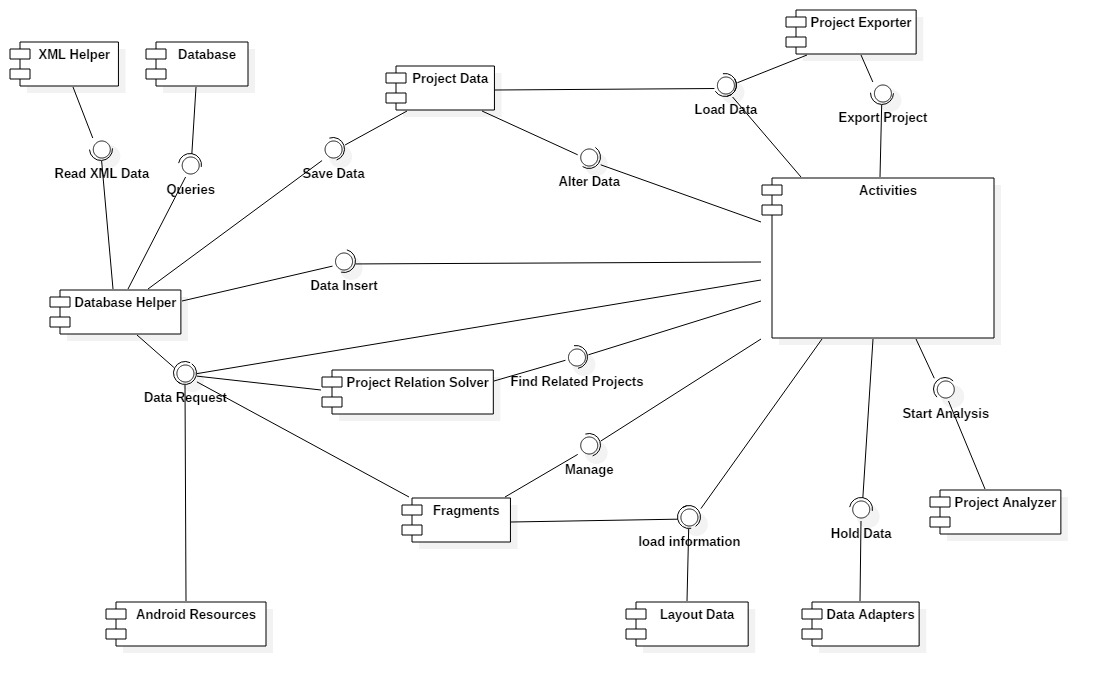
\includegraphics[width=14cm]{images/components.jpg} 
	\caption{- Component Diagram} 
	\label{fig:components}
\end{figure}

\section{Components}

This section describes the most important components from figure \ref{fig:components} in detail and what concepts they inherit. 

\subsection{Database Helper}

The \textit{Database Helper} component is responsible for accessing the database, where all project informations are stored. Every Class that needs access to the database should only create an object of this component and can read or write data to the database.\\
The component should contain name and path to the database and allow the initialization of the database. As described in fig. \ref{fig:sequenceDBHelper}, with the message \textit{Open Constructor}, an initialization of the database should be done in the constructor of classes that need access to it. This will opens the \textit{SQLite} database and ensures that request on the database can be performed and no error occurs while accessing a non initialized database. All functionalities that are working on the database are in fig. \ref{fig:sequenceDBHelper} combined to the message \textit{Using Class} and combines the three categories for working with the database \textit{SELECT}, \textit{ALTER} and \textit{DELETE}.\\ 
For requesting data from the database a Java class has to send a request with the table name and the selection criteria to the Database Helper. This will be transformed into a query which is send to the database. Before sending this data back to the calling Java class the database Helper has to transform the \textit{SQL} query result into readable information. Editing existing informations in the database is done with the message \textit{Alter Existing Data} and the parameters table name and data to be edited. Before sending data to the database the \textit{Database Helper} has to prepare it to insert them in the right column of the table. This query will return true if inserting was successful or false if it was not. Last message option is \textit{Delete Data} which will delete entries from the database. The parameter \textit{tablename} and \textit{Data ID} are the identifiers for a selected entry. Before deleting data from the database the \textit{Database Helper} has to check if there are any other tables depending to the selected entry and have to ensure that they are deleted too if necessary. After all depending tables are identified the Database Helper will send the delete query to the database. It will then return a boolean value for the deletion process which is forwarded to the Java Class.

\begin{figure}[h] 
	\centering 
	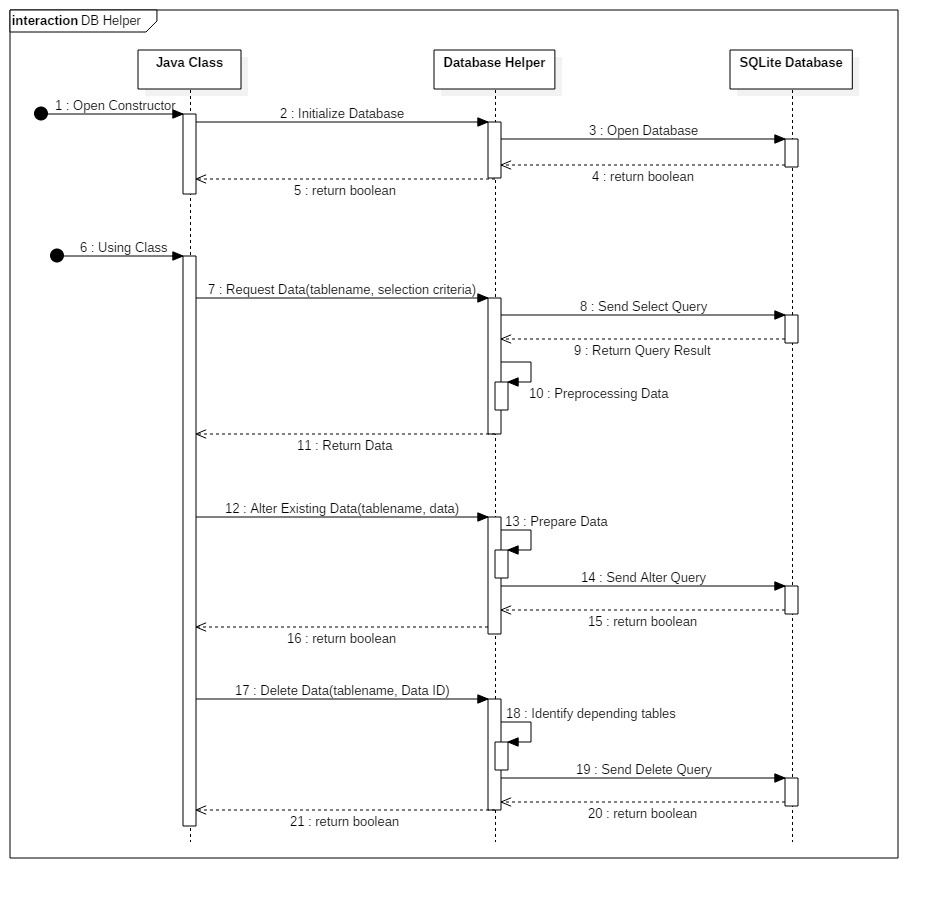
\includegraphics[width=14cm]{images/DBHelper.jpg} 
	\caption{- DB Helper Sequence Model} 
	\label{fig:sequenceDBHelper}
\end{figure}

\subsection{Project Data}

The \textit{Project Data} component was created to make combine all data of a project from the database and make it accessible for other classes. It contains \textit{Name}, \textit{Description}, \textit{Creation Date} and \textit{Estimation Technique} at the first level of the component. This makes it possible to get a fast overview of the different projects in the application. For estimation specific purposes the \textit{Estimation Items} and \textit{Influence Factor} are minor components for the project data and differ from the projects estimation technique. The \textit{Properties} are also a minor component to build a module-based structure. As the output information of estimation techniques is the same, the main component contains the amount of \textit{Estimated Man Days} for the project. If the project is completed the \textit{Final Man Days} represent the time the project really took. This value is important to improve future estimations as described in section \ref{adjustedEstimationProcess}, where the improvement process is specified.
\begin{figure}[h] 
	\centering 
	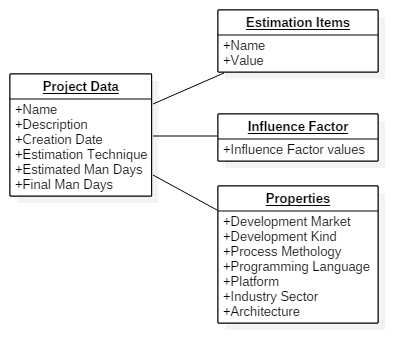
\includegraphics[width=10cm]{images/ObjectDiagramProject.png} 
	\caption{- Object Diagram for Projects} 
	\label{fig:objectDiagrammProject}
\end{figure}

\subsubsection{Project Properties}

This minor component contains the information that is needed for the \textit{Project Relation Solver} in section \ref{projectRealtionSolver}. It is a data component which stores all properties that allows reading and editing. Access to is granted to the properties only through the project component which assures that a property is bound to a project.\\

\subsubsection{Estimation Items}

All items for the estimation are in the \textit{Estimation Items} components. These are the items for an estimation technique that are responsible for the estimation itself. In the \textit{Function Point} estimation for example, these items calculate the value \textit{E1} from the equation \ref{fp:E1}.\\

\subsubsection{Influence Factors}

This component contains all informations for \textit{Influence Factors}. These are \textit{name}, \textit{chosen value} and the \textit{limit} for the value. This component is also responsible for preprocessing the influence factor for usable information at the calculation of the estimation. In the Function Point estimation for example, this component calculated the value \textit{E2} and \textit{E3} that are described in section \ref{fp:classificationInfluence}.\\

\subsection{Project Relation Solver}\label{projectRealtionSolver}

To fulfill the target \textit{T06} from section \ref{objectives}, this component is responsible to find related project. The point of this component is to compare already existing projects with a selected one. This should help the user to get an overview of how similar projects were estimated. Furthermore the \textit{Project Relation Solver} should allow to transfer the estimation from a related project to the selected to have an estimation where the user can build on.\\
The \textit{Project Relation Solver} compares therefor an selected project with every other available project from the database. This comparison is made in mainly three steps.
\paragraph*{1. Determination of the Property Distances}
asdasdasd
\paragraph*{2. Determination of the Total Distance}
asdasdasd
\paragraph*{3. Calculation of the Relation}
asdasdasd\\
asdasd

\subsection{Project Analyzer}

Aufbau der Analyze der Projekte, Wie die Graphen vorgestellt. Sinn davon

\subsection{Minor Components}

Export, statistic, Help DB, Feedback, Project Filter, accessing resources


\section{Database design}

Vorheriges Design der zentralen Datenbank. Wichtig um die Klassen anzupassen und vorher schon mit wichtigen Daten zu füllen

\subsection{Project Database}

Datenbank für alle Projekte, Eigenschaften, Einflussfaktoren

\subsubsection{Project Properties}

Welche Tabellen gibt es. Wichtige Tabellen, Aufbau der Tabellen und Grund

\subsubsection{Influence Factors}

Wie die Einflussfaktoren Aufgebaut, was ist der Gedanke dazu?

\subsubsection{Projects}

Wie sind Projekte gespeichert, Aufteilung in Projekt, Projektdetails und zugehörige Tabellen, wie die Schätzung Organisiert und wie der Zugriff auf die Elemente

\subsection{Userinformation Database}

Datenbank für Spätere Synchronisation und Userinformationen vom Server, Konzept dazu

\section{User Interface}

\subsection{Projects Overview}

Anordnung der Projekte, Wichtige Informationen zum sehen, Filtern und Suchen nach Projekten

\subsection{Project Creation}

Komponente zur korrekten Erstellung von Projekten, Geführte Eingabe, Korrekte Erstellung von Projekten in der DB, Swipe Funktion

\subsection{Estimate Function Point Project}

Aufbau der Schätzung, Umwandlung von Tabelle in App

\subsection{Influence Factors}

Aufbau der EInflussfaktoren, Neue anlengen

\subsection{Analysis}

Wie die Analyse aufgebau und was soll diese bringen?

\section{Adjusted Estimation Process}\label{adjustedEstimationProcess}


\subsection{Continuous Improvement of the Estimation}

